\setcounter{equation}{0}
\section{Non-inertial frames of reference}

	A reference frame (e.g. a coordinate system) in which Newton's first law of motion does not hold good, is known as a \emph{non-inertial frame of reference}.
	
	All frames of reference having an accelerated motion with respect to an inertial frame are non-inertial frames of reference.
	
	\begin{figure}[h!]
		\centering
		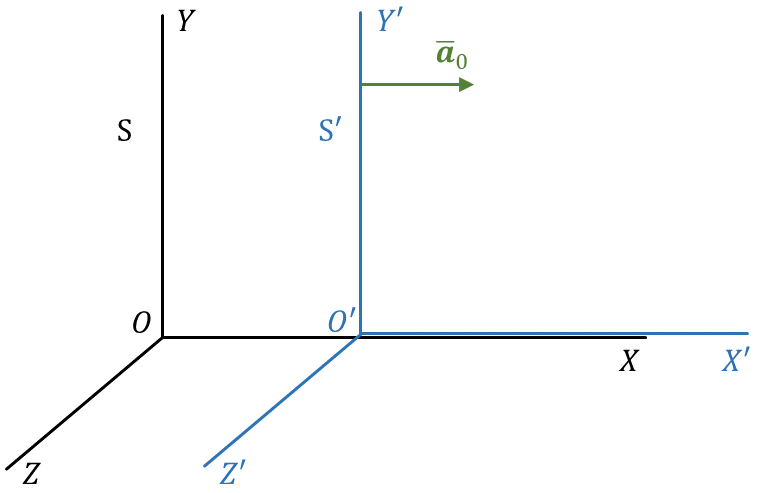
\includegraphics[width=0.5\textwidth]{figures/fig_non-inertial-frame.png}
	\end{figure}
	
	In the above figure, $S$ is an inertial frame. Another frame $S'$ is moving with an acceleration $\vb{a}_0$ with respect to frame $S$. Here the frame $S'$ is a non-inertial frame of reference.
	
	\begin{figure}[h!]
		\centering
		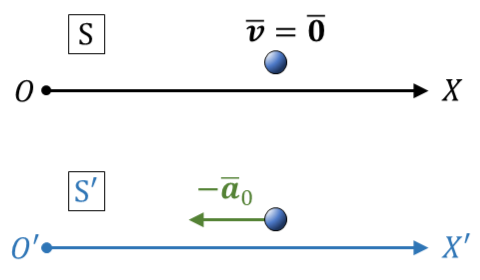
\includegraphics[width=0.4\textwidth]{figures/fig_non-inertial_rest.png}
	\end{figure}
	If a particle of mass $m$ is at rest with respect to the frame $S$, then it would appear to have an acceleration $-\vb{a}_0$ with respect to the frame $S'$.
	
	From Newton's second law of motion, with respect to $S'$, it appears as if some pseudo-force
	\begin{align}
		\vb{F}_p=-m\vb{a}_0 \label{eqn:non-iner:pseudo}
	\end{align}
	is acting on the particle.
	
	\begin{figure}[h!]
		\centering
		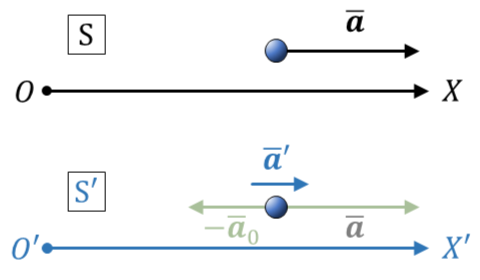
\includegraphics[width=0.4\textwidth]{figures/fig_non-inertial_accl.png}
	\end{figure}
	Suppose now that the particle has an acceleration $\vb{a}$ with respect to the frame $S$. Then the force acting on it in $S$ is
	\begin{align}
		\vb{F}&=m\vb{a} \label{eqn:non-iner:force-S}
	\end{align}
	
	The acceleration of the particle with respect to the non-inertial frame $S'$ would be
	\begin{align*}
		\vb{a}'&=\vb{a}-\vb{a}_0
	\end{align*}
	
	Then from Newton's second law of motion, the force acting on the particle with respect to $S'$ would be
	\begin{align}
		\vb{F}'&=m\vb{a}' \nonumber \\
			&=m\qty(\vb{a}-\vb{a}_0) \nonumber \\
			&=m\vb{a}-m\vb{a}_0 \nonumber \\
		\implies\Aboxed{\vb{F}&=\vb{F}+\vb{F}_p}\qq{[using eqns. (\ref{eqn:non-iner:pseudo}) and (\ref{eqn:non-iner:force-S})]} \label{eqn:non-iner:force-S-p}
	\end{align}
	
	Equations (\ref{eqn:non-iner:pseudo}) and (\ref{eqn:non-iner:force-S-p}) show that, regardless of whether a force is acting on a particle in the inertial frame, a pseudo-force of $\vb{F}_p=-m\vb{a}_0$ always seems to be acting on the particle in the non-inertial frame of reference.
	
	Such pseudo-forces, which arise due to the accelerated motion of a non-inertial frame of reference, are known as \emph{fictitious forces}.
	
	\subsection{Rotating coordinate systems}
	
		\setcounter{equation}{0}
		\subsubsection*{Rate of change of a rotating vector}
			\setwrappadding
			\begin{wrapfigure}[16]{r}{0.35\textwidth} % 'r' for right side, width is 35% of text width
				\centering
				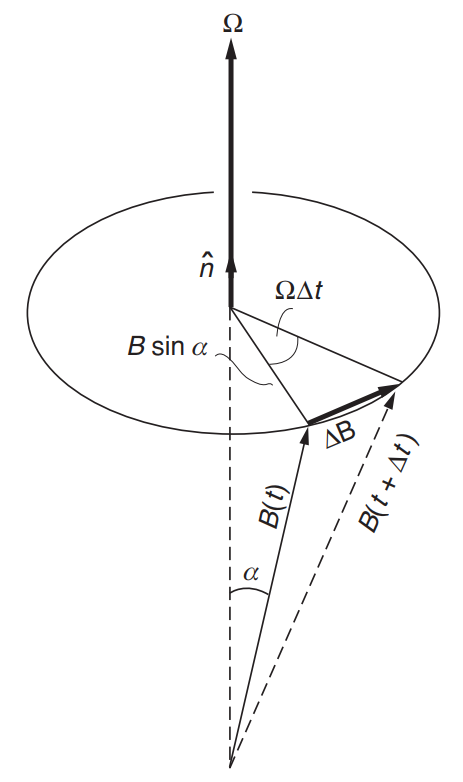
\includegraphics[width=0.98\linewidth]{figures/fig_rotating-vector-rate}
			\end{wrapfigure}
			Consider an arbitrary vector $\vb{B}$ which is precessing at an angular frequency of $\Omega$ about an arbitrary axis lying in the $\vu{n}$ direction as shown in the figure.
			\resetwrappadding
			
			Then the angular velocity vector is $\vb{\Omega}=\Omega\vu{n}$. Let $\alpha$ be the angle between the vectors $\vb{B}$ and $\vb{\Omega}$. At times $t$ and $t+\Delta t$, we have the vectors $\vb{B}(t)$ and $\vb{B}(t+\Delta t)$ respectively. The tip of $\vb{B}$ sweeps out a circular path with radius $B\sin{\alpha}$ and the plane of the circle is perpendicular to $\vu{n}$.
			
			During time $\Delta t$ the tip of $\vb{B}$ swings through an angle of $\Omega\Delta t$. Consequently, the tip of $\vb{B}$ moves by an amount $\Delta B$, where
			\begin{align*}
				\Delta B\approx\qty(B\sin{\alpha})\Omega\Delta t
			\end{align*}
			
			Then the rate of change of $\vb{B}$ has the magnitude
			\begin{align*}
				\dv{B}{t}&=\lim_{\Delta t\to 0}{\dfrac{\Delta B}{\Delta t}} \\
					&=\lim_{\Delta t\to 0}{\dfrac{\qty(B\sin{\alpha})\Omega\Delta t}{\Delta t}} \\
				\implies\dv{B}{t}&=\Omega B\sin{\alpha}
			\end{align*}
			
			From the figure, we find that $\Delta\vb{B}$ is perpendicular to both $\vb{B}$ and $\vu{n}$. Hence $\dv{\vb{B}}{t}$ is also perpendicular to both $\vb{B}$ and $\vu{n}$. We also find that $\Omega B\sin{\alpha}=|\vb{\Omega}\cross\vb{B}|$. Therefore,
			\begin{align}
				\dv{\vb{B}}{t}&=\vb{\Omega}\cross\vb{B} \label{eqn:dB-dt}
			\end{align}
			Equation (\ref{eqn:dB-dt}) is true for any vector $\vb{B}$ that undergoes pure rotation around an axis $\vu{n}$ at a rate $\Omega$.
			
		\subsubsection*{Time derivative of a vector in a rotating frame}
			We consider a frame of reference $S'$ that is rotating with respect to an inertial frame $S$. Let the base vectors be $(\vu{x},\vu{y},\vu{z})$ in the inertial frame and $(\vu{x}',\vu{y}',\vu{z}')$. Then some arbitrary vector $\vb{C}$ can be expressed in either frames as
			\begin{align}
				\vb{C}&=\vu{x}C_x+\vu{y}C_y+\vu{z}C_z=\vu{x}'C_x'+\vu{y}'C_y'+\vu{z}'C_z' \label{eqn:C-iner-rot}
			\end{align}
			The time derivative of $\vb{C}$ in the inertial frame is
			\begin{align}
				\qty(\dv{\vb{C}}{t})_\text{in}&=\vu{x}\dv{C_x}{t}+\vu{y}\dv{C_y}{t}+\vu{z}\dv{C_z}{t} \label{eqn:dC-dt-in}
			\end{align}
			And the time derivative of $\vb{C}$ in the rotating frame is
			\begin{align}
				\qty(\dv{\vb{C}}{t})_\text{rot}&=\vu{x}'\dv{C_x'}{t}+\vu{y}'\dv{C_y'}{t}+\vu{z}'\dv{C_z'}{t} \label{eqn:dC-dt-rot}
			\end{align}
			
			Now the base vectors $(\vu{x}',\vu{y}',\vu{z}')$ in the rotating frame all rotate with the same angular velocity $\vb{\Omega}$. Hence, in equation (\ref{eqn:dB-dt}), replacing $\vb{B}$ with $\vu{x}'$, $\vu{y}'$ and $\vu{z}'$, we have
			\begin{align}
				\dv{\vu{x}'}{t}=\vb{\Omega}\cross\vu{x}',\quad\dv{\vu{y}'}{t}=\vb{\Omega}\cross\vu{y}',\quad\dv{\vu{z}'}{t}=\vb{\Omega}\cross\vu{z}' \label{eqn:dxyz-dt}
			\end{align}
			
			Taking the time derivative of equation (\ref{eqn:C-iner-rot}) gives us
			\begin{align}
				\dv{t}\qty(\vu{x}C_x+\vu{y}C_y+\vu{z}C_z)&=\dv{t}\qty(\vu{x}'C_x'+\vu{y}'C_y'+\vu{z}'C_z') \nonumber\\
				\implies\vu{x}\dv{C_x}{t}+\vu{y}\dv{C_y}{t}+\vu{z}\dv{C_z}{t}&=\qty(\vu{x}'\dv{C_x'}{t}+C_x'\dv{\vu{x}'}{t})+\qty(\vu{y}'\dv{C_y'}{t}+C_y'\dv{\vu{y}'}{t})+\qty(\vu{z}'\dv{C_z'}{t}+C_z'\dv{\vu{z}'}{t}) \nonumber\\
				\implies\vu{x}\dv{C_x}{t}+\vu{y}\dv{C_y}{t}+\vu{z}\dv{C_z}{t}&=\qty(\vu{x}'\dv{C_x'}{t}+\vu{y}'\dv{C_y'}{t}+\vu{z}'\dv{C_z'}{t})+\qty(C_x'\dv{\vu{x}'}{t}+C_y'\dv{\vu{y}'}{t}+C_z'\dv{\vu{z}'}{t}) \nonumber\\
				\implies\qty(\dv{\vb{C}}{t})_\text{in}&=\qty(\dv{\vb{C}}{t})_\text{rot}+\qty(C_x'\vb{\Omega}\cross\vu{x}'+C_y'\vb{\Omega}\cross\vu{y}'+C_z'\vb{\Omega}\cross\vu{z}') \qq{[Using eqns. (\ref{eqn:dC-dt-in}), (\ref{eqn:dC-dt-rot}), (\ref{eqn:dxyz-dt})]} \nonumber\\
				\implies\qty(\dv{\vb{C}}{t})_\text{in}&=\qty(\dv{\vb{C}}{t})_\text{rot}+\vb{\Omega}\cross\qty(\vu{x}'C_x'+\vu{y}'C_y'+\vu{z}'C_z') \nonumber\\
				\implies\qty(\dv{\vb{C}}{t})_\text{in}&=\qty(\dv{\vb{C}}{t})_\text{rot}+\vb{\Omega}\cross\vb{C} \qq{[Using eqn. (\ref{eqn:C-iner-rot})]} \label{eqn:dC-dt-iner-rot}
			\end{align}
			
		\subsubsection{Velocity and acceleration in a rotating frame}
			In equation (\ref{eqn:dC-dt-iner-rot}), if we set $\vb{C}$ as the position vector of the particle, i.e. $\vb{C}=\vb{r}$, then we have
			\begin{align}
				\qty(\dv{\vb{r}}{t})_\text{in}&=\qty(\dv{\vb{r}}{t})_\text{rot}+\vb{\Omega}\cross\vb{r} \nonumber\\
				\implies\vb{v}_\text{in}&=\vb{v}_\text{rot}+\vb{\Omega}\cross\vb{r} \label{eqn:vin-vrot}\\
				\implies\Aboxed{\vb{v}_\text{rot}&=\vb{v}_\text{in}-\vb{\Omega}\cross\vb{r}} \label{eqn:vrot-vin}
			\end{align}
			where $\vb{v}_\text{in}$, $\vb{v}_\text{rot}$ are the velocities of the particle measured with respect to $S$ and $S'$ respectively.
			
			Again, in equation (\ref{eqn:dC-dt-iner-rot}), if we set $\vb{C}$ as the velocity of the particle in the inertial frame, i.e. $\vb{C}=\vb{v}_\text{in}$, then we have
			\begin{align}
				\qty(\dv{\vb{v}_\text{in}}{t})_\text{in}&=\qty(\dv{\vb{v}_\text{in}}{t})_\text{rot}+\vb{\Omega}\cross\vb{v}_\text{in} \nonumber\\
					&=\qty[\dv{t}\qty(\vb{v}_\text{rot}+\vb{\Omega}\cross\vb{r})]_\text{rot}+\vb{\Omega}\cross\qty[\vb{v}_\text{rot}+\vb{\Omega}\cross\vb{r}] \qq{[Using eqn. (\ref{eqn:vin-vrot})]} \nonumber\\
					&=\qty(\dv{\vb{v}_\text{rot}}{t})_\text{rot}+\vb{\Omega}\cross\underbrace{\qty(\dv{\vb{r}}{t})_\text{rot}}_{=\vb{v}_\text{rot}}+\vb{\Omega}\cross\vb{v}_\text{rot}+\vb{\Omega}\cross\qty(\vb{\Omega}\cross\vb{r}) \nonumber\\
				\implies\underbrace{\qty(\dv{\vb{v}_\text{in}}{t})_\text{in}}_{=\vb{a}_\text{in}}&=\underbrace{\qty(\dv{\vb{v}_\text{rot}}{t})_\text{rot}}_{=\vb{a}_\text{rot}}+\vb{\Omega}\cross\vb{v}_\text{rot}+\vb{\Omega}\cross\vb{v}_\text{rot}+\vb{\Omega}\cross\qty(\vb{\Omega}\cross\vb{r}) \nonumber\\
				\implies\vb{a}_\text{in}&=\vb{a}_\text{rot}+2\vb{\Omega}\cross\vb{v}_\text{rot}+\vb{\Omega}\cross\qty(\vb{\Omega}\cross\vb{r}) \nonumber\\
				\implies\Aboxed{\vb{a}_\text{rot}&=\vb{a}_\text{in}-2\vb{\Omega}\cross\vb{v}_\text{rot}-\vb{\Omega}\cross\qty(\vb{\Omega}\cross\vb{r})} \label{eqn:arot-ain}
			\end{align}
			
			Equations (\ref{eqn:vrot-vin}) and (\ref{eqn:arot-ain}) respectively give us the velocity and acceleration of the particle as observed from the rotating frame of reference.
			
		\subsubsection{Fictitious forces in a rotating frame}
			With respect to a rotating frame of reference, Newton's second law of motion gives us the net force acting on a particle of mass $m$ to be
			\begin{align}
				\vb{F}_\text{rot}&=m\vb{a}_\text{rot} \label{eqn:F-rot}
			\end{align}
			
			Inserting equation (\ref{eqn:arot-ain}) into equation (\ref{eqn:F-rot}) we obtain
			\begin{align}
				\vb{F}_\text{rot}&=m\qty[\vb{a}_\text{in}-2\vb{\Omega}\cross\vb{v}_\text{rot}-\vb{\Omega}\cross\qty(\vb{\Omega}\cross\vb{r})] \nonumber\\
					&=m\vb{a}_\text{in}-2m\vb{\Omega}\cross\vb{v}_\text{rot}-m\vb{\Omega}\cross\qty(\vb{\Omega}\cross\vb{r}) \nonumber\\
				\implies\vb{F}_\text{rot}&=\vb{F}-2m\vb{\Omega}\cross\vb{v}_\text{rot}-m\vb{\Omega}\cross\qty(\vb{\Omega}\cross\vb{r}) \label{eqn:F-rot-01}
			\end{align}
			
			On the RHS of equation (\ref{eqn:F-rot-01}), we refer to all the terms as
			\begin{itemize}
				\item \emph{Actual force:}
				$\vb{F}=m\vb{a}_\text{in}$\\
				This is the force on the particle as observed from the inertial frame of reference.
				
				\item \emph{Centrifugal force:} $\vb{F}_\text{centrifugal}=-m\vb{\Omega}\cross\qty(\vb{\Omega}\cross\vb{r})$\\
				This fictitious force is perpendicular to the axis of rotation and is directed radially outward.
				
				\item \emph{Coriolis force:} $\vb{F}_\text{Coriolis}=-2m\vb{\Omega}\cross\vb{v}_\text{rot}$\\
				This fictitious force is an apparent sideways force that deflects a moving object perpendicularly to both the direction of rotation and the object's own motion.
			\end{itemize}
			
			Therefore, we can write the force on the particle in a rotating frame as
			\begin{align*}
				\vb{F}_\text{rot}&=\vb{F}+\vb{F}_\text{centrifugal}+\vb{F}_\text{Coriolis} \\
				\qq{or,}\vb{F}_\text{rot}&=\vb{F}_\text{fict}
			\end{align*}
			where the total fictitious force due to the rotating frame is
			\begin{align*}
				\vb{F}_\text{fict}&=\vb{F}_\text{centrifugal}+\vb{F}_\text{Coriolis}
			\end{align*}